\documentclass{article}
\usepackage[utf8]{inputenc}
\usepackage{authblk}
\usepackage{setspace}
\usepackage[margin=1.25in]{geometry}
\usepackage{graphicx}
\usepackage{xcolor}
\usepackage{float}
\graphicspath{ {./figures/} }
\usepackage{amsmath,amssymb,amsfonts}
\usepackage{booktabs}
\usepackage{natbib}
\usepackage{hyperref}
\hypersetup{colorlinks=true, linkcolor=blue, citecolor=blue, urlcolor=blue}

\title{\textbf{Central Bank Balance Sheet Growth and Subsequent US Equity Returns}}
\author[1]{SIQuant Research}
\affil[1]{Hypothesis $\times$ Quant}
\date{\today}
\onehalfspacing

\begin{document}
\maketitle

\begin{abstract}
\noindent \textbf{Hypothesis:} $H_0$: the four-week change in Federal Reserve total assets has no predictive power for the S\&P 500 return over the next 20 sessions; $H_1$: the slope is positive \\
\textbf{Data:} 519 weekly observations, 2016-10-24 to 2026-09-25; information date set to the Friday after the Thursday release \\
\textbf{Method:} OLS with Newey--West HAC errors (8 lags) and a 2,000-draw circular-shift placebo; the decision needs both one-sided $p<0.05$ \\
\textbf{Results:} $\beta=0.256$ (HAC $t=4.53$, $p=0.0000$; placebo $p=0.0085$), $R^2=0.0288$; mean forward return 0.94\% after expansion and 1.05\% after contraction; without 2020 the slope is 0.262 ($t=1.19$). \\
\textbf{Research decision:} \colorbox[rgb]{0.10,0.50,0.20}{\textcolor{white}{\textbf{\,ACCEPTED\,}}}
\end{abstract}

\section{Design}
Liquidity provision by central banks is often linked to risk-asset performance \citep{lewis2019monetary}. The H.4.1 release is public on Thursday afternoon, so the earliest tradable close is Friday; the outcome window starts from that close. The signal is the four-week log change in WALCL.

\section{Results}
\begin{figure}[H]
\centering
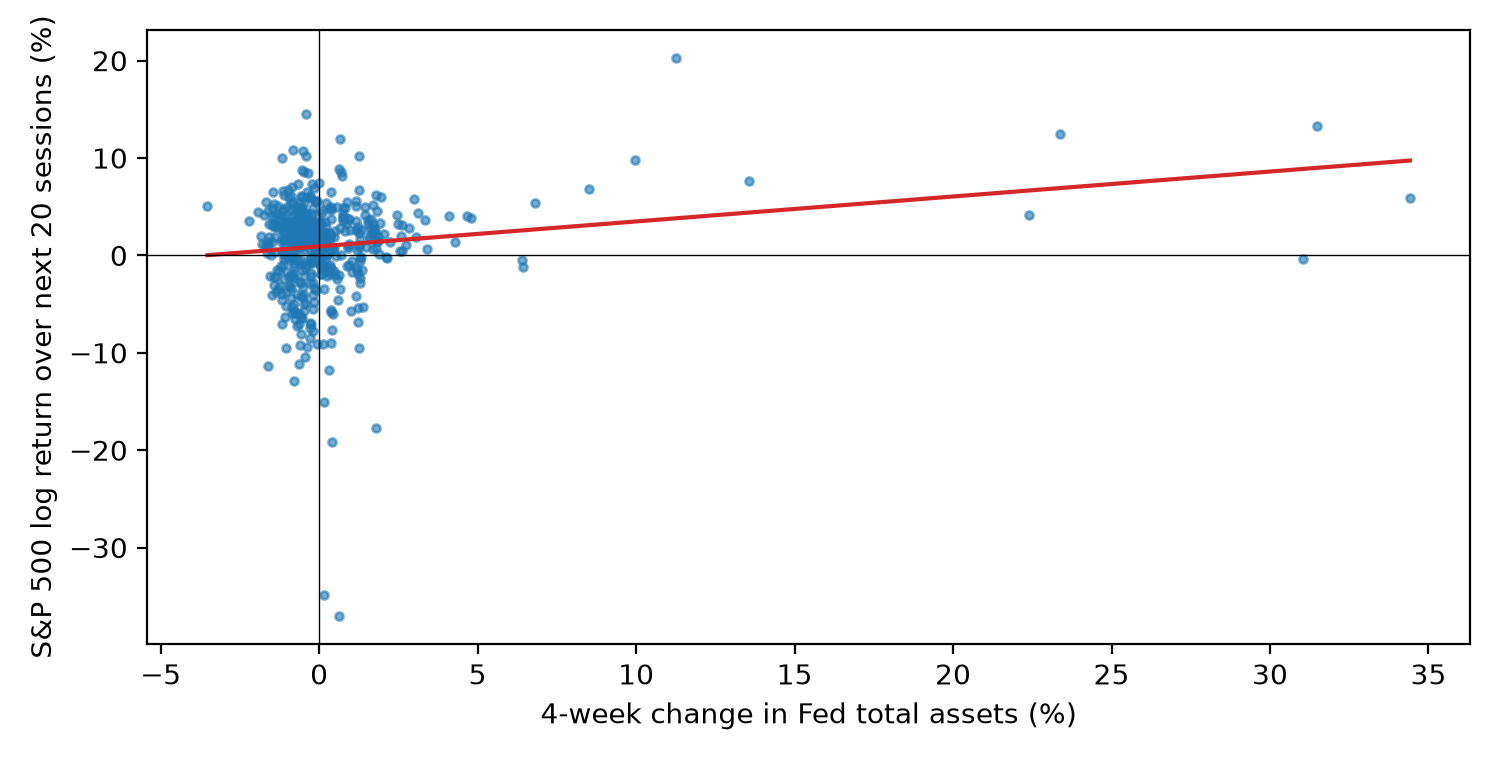
\includegraphics[width=0.8\textwidth]{fig1_fed_assets_vs_forward_return.png}
\caption{Four-week balance-sheet change against the next 20-session S\&P 500 return.}
\end{figure}

Excluding the 2020 episode the slope is 0.262 (HAC $t=1.19$); mean 20-session returns after expansion and contraction weeks are 0.94\% and 1.05\%, so the sign of the change alone carries little information and the pooled slope depends on large balance-sheet moves.

\section{Limitations}
The sample contains one expansion (2020--21) and one contraction (2022--) regime, so effective independent observations are very few. Balance-sheet growth is endogenous to market stress. Reserve and Treasury General Account dynamics are not modelled.


\bibliographystyle{plainnat}
\bibliography{references}

\end{document}
